\documentclass[10pt,a4paper]{article}
% This file compiles fine with pdflatex,
% (here: TeX Live 2013/Frankfurt Institute for Advanced Sciences)
\usepackage[utf8]{inputenc}
\usepackage{hyperref}
\hypersetup{linktocpage}
\usepackage[american]{babel}
\usepackage{amsmath} % xrightarrow, ...
\usepackage{cite}
\usepackage{units} % nicefrac
\usepackage{datetime} % time and \date
\usepackage{caption}
\usepackage{subcaption} % subfigures
\usepackage{graphicx} % pictures
\usepackage{tabularx} % tables
\usepackage{a4wide} % more space on sheets
\usepackage{amssymb} % symbols
\usepackage{array} % tables
\usepackage{booktabs} % better tables
\usepackage{floatrow} % caption beside image
\usepackage{wrapfig} % wrapping (floating)
\usepackage[toc,page]{appendix}

\usepackage[usenames,dvipsnames]{color} % more colors

% highlighting
\usepackage{xcolor}
\newcommand{\highlight}[1]{%
%  \colorbox{green!30}{$\displaystyle#1$}
   \fcolorbox{green}{green!30}{$\displaystyle#1$}%
}


%%% highlight in align-umgebung
%%% http://tex.stackexchange.com/questions/13681/highlight-an-equation-within-an-align-environment  
% Usage: \alignedbox{links}{rechts}
\usepackage{calc}
\newlength\dlf
\newcommand\alignedbox[2]{
  % #1 = before alignment
  % #2 = after alignment
  &
  \begingroup
  \settowidth\dlf{$\displaystyle #1$}
  \addtolength\dlf{\fboxsep+\fboxrule}
  \hspace{-\dlf}
  \fcolorbox{green}{green!30}{$\displaystyle #1 #2$}
  \endgroup
}
  
% TODO boxes
% Alternative dazu (gut fuer Seitenanmerkungen):
% http://tex.stackexchange.com/a/73418/49958
\usepackage[draft,colorinlistoftodos]{todonotes}   % notes showed

% Bibliography
\bibliographystyle{ieeetr}

% Colors (only used by hyperref)
\usepackage{color}
\definecolor{darkblue}{rgb}{0,0,.6}
\definecolor{darkred}{rgb}{.1,0,0}
\definecolor{darkgreen}{rgb}{0,.5,0}

% Hyperref for PDF
\hypersetup{
    pdftitle={Master Physik bei Nicolini, Calc writeup},
    pdfauthor={Sven Köppel},
    pdfsubject={master},
    pdfkeywords={physik} {master} {uni} {frankfurt} {fias},
    colorlinks=true,        % test: stat gerahmten Links
    linkcolor=red,          % color of internal links
    citecolor=darkgreen,    % color of links to bibliography
    filecolor=darkred,      % color of file links
    urlcolor=cyan           % color of external links
}

\title{Another modified GUP in Extra Dimensions}
\author{Marco Knipfer, Sven Köppel \\
\texttt{\{knipfer, koeppel\}@fias.uni-frankfurt.de}}
\date{Generation date: \today, \currenttime}

\begin{document}
\maketitle

% shorthands for differentials, etc
\renewcommand{\d}{\mathrm{d}}
\newcommand{\dd}[2]{\frac{\mathrm{d} #1}{\mathrm{d} #2}}
\newcommand{\pp}[2]{\frac{\partial #1}{\partial #2}}
\newcommand{\dann}{$\rightarrow~$}
\newcommand{\CA}{ {\cal A}}
\newcommand{\C}[1]{ {\cal #1} }
\newcommand{\mn}{_{\mu\nu}}
\newcommand{\bv}[1]{ \mathbf{ #1 } } % bold vector

\newcommand{\rb}{\frac{r}{\sqrt{\beta}}}
\newcommand{\rbb}{\nicefrac{r}{\sqrt{\beta}}}

% colored symbols:
% http://tex.stackexchange.com/questions/85033/colored-symbols
\newcommand*{\mathcolor}{}
\def\mathcolor#1#{\mathcoloraux{#1}}
\newcommand*{\mathcoloraux}[3]{%
  \protect\leavevmode
  \begingroup
    \color#1{#2}#3%
  \endgroup
}
% In Text: $a\textcolor{red}{\ast}b$
% In Math: $a\mathcolor{red}{\ast}b$
\newcommand{\redmin}{\mathcolor{red}{-}}
\newcommand{\redplus}{\mathcolor{red}{+}}
\newcommand{\pn}{\mathcolor{OliveGreen}{+ n}}
\newcommand{\n}{ {\mathcolor{OliveGreen}{n}} }

\begin{abstract}
We present here another modified GUP that exposes cold remnants in any number of dimensions, we will call that approach ``backward-modified'' since we start with the metric and derive the nonlocal operator which is tested if it is a good GUP modification or not (it turns out it is not).

We also discuss the last kind of ``naively'' modified GUP from Svens July 6, 2014 proposal in terms of a long-distance (i.e. Schwarzschild) expansion.

This document contains ideas and thoughts developed by Marco and Sven while the DPG physics school \emph{GR@99} in Bonn/Bad Honnef, Sept 2014.

This document is written in the context of the currently prepared paper \textit{Self-Completeness and the Generalized Uncertainty Principle in Extra Dimensions} calculated by Maximiliano Isi and Marco Knipfer \cite{work}.
\hfill\textit{Internal working title:} \textsc{Calc19}
\end{abstract}


\tableofcontents

%\listoftodos

\newpage

%%%%%%%%%%%%% BEGIN OF CONTENT %%%%%%%%%%%%%%
\section{Another modified GUP (``backward-modified'')}\label{sec:1}
We present a way to compute the GUP function $f(\bv p)$ in the Kempf notation
\begin{equation}
\Delta x \Delta p \geq \frac{\hbar}{2} \left( 1 + f(\bv p) \right)
\end{equation}
in $N$ spatial dimensions. For $N=3$ and $f(\bv p)=\beta \bv p^2$, in 2013 Max et al \cite{isi2013} derived the metric
\begin{equation}\label{eq:metric3}
g_{00} = 1 - \frac{2GM}{r} \gamma(2; \rbb)
\end{equation}
with the lower gamma function $\gamma(n,z)$. Marco and Max did not found remnants for some big $N$ any more, so I proposed a modified GUP $f(p)=L^{N-1}p^{N-1}$ which produced a repulsive gravitational potential which discussion is proceeded in section \ref{sec:2}.

In this section, we search for another modified GUP, in a ``reverse'' fashion by starting from the metric: With an ``educated guess'' while looking at metric \eqref{eq:metric3}, we propose an $N$-dimensional extension by means of
\begin{equation}\label{eq:metric}
\highlight{
g_{00} = 1 - \frac{2GM}{r^{N-2}} \gamma(N-1; \rbb).
}%eoh
\end{equation}

We checked that this metric exposes remnants in any dimension $N$ with appropriate masses $M_*$, as given in table \ref{table:Length-scales}. See figure \ref{fig:g00} for the plot of $g_{00}$ for an arbitrary dimension $N$.

\begin{table}[b!]
\begin{center}
\begin{tabular}{ccccccccc}
\firsthline
 $n$ & 0 & 1 & 2 & 3 & 4 & 5 & 6 & 7 \\
 \hline
 $r_0$ & 1.79328 & 1.45123 & 1.31433 & 1.24065 & 1.19472 & 1.1634 & 1.1407 & 1.1235 \\
 $M_*$ & 1.67546 & 2.9412 & 4.24808 & 5.57428 & 6.9109 & 8.25373 & 9.60055 & 10.9501 \\
   \hline
\end{tabular}
\end{center}
\caption{Minimal length $r_0=L$ and memnant masses in 4d Planck units for the ``backward-modified'' GUP}\label{table:Length-scales}
\end{table}

\begin{figure}
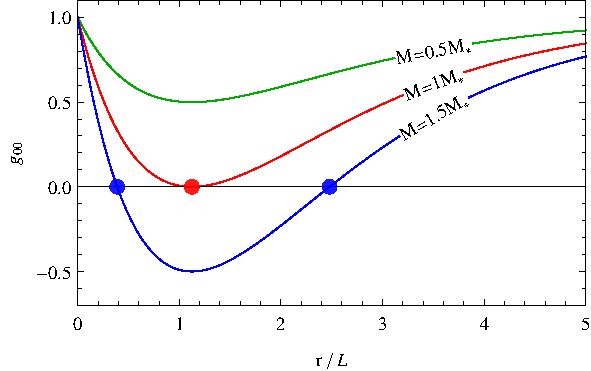
\includegraphics[scale=1]{figures/g00_n7.pdf}
\caption{The remnant picture for $n=7$ ($N=10$) for our modified GUP as given in equation \eqref{eq:metric}, here $M_*=10.95 M_P$ like estimated in table \ref{table:Length-scales}. The plot basically looks the same in any number of dimensions.}\label{fig:g00}
\end{figure}

\clearpage
\subsection{Derivation of the stress tensor}
We now derive the nonlocal operator $\C A^{-2}$ from our modified metric \eqref{eq:metric}. To do so, we identify the modified mass $\C M$ of the Black hole with event horizon $r_H$ by
\begin{equation}
g_{00} = 1 - \frac{2G \C M(r_H)}{r_H^{N-2}}, \quad
\C M(r_H) = M \gamma(N-1; \nicefrac{r_H}\beta).
\end{equation}
On the other hand, it is linked to the mass density by the full space integration
\begin{equation}
\C M(R) = \int_{\C B(R)} \d^N r \C T^0_0(r) =
\int_0^R \d r~r^{N-1} \C T^0_0(r) A_{N-2}
\end{equation}
with $\C B(R)$ being the ball with volume $R$, $A_{N-2}$ the surface area of that ball and $\C T^0_0$ the mass density (first entry of modified energy momentum tensor) we are looking for. We compute it by deriving the gamma function:
\begin{equation}
\C T^0_0(r) = \frac{\partial_r \C M(r)}{r^{N-1} A_{N-2}} = \frac{M}{r^{N-1} A_{N-2}} \partial_r \gamma(N-1; \rbb).
\end{equation}
Inserting the definition of the gamma function, the derivate is given by
\begin{equation}
\gamma(N-1; \rbb) = \int_0^{\rbb} t^{N-2} e^{-t} \d t
\quad\Rightarrow\quad
 \partial_r \gamma(N-1; \rbb) = (\rbb)^{N-2} e^{-\rbb},
\end{equation}
so we determined the mass density for the modified metric to
\begin{equation}
\highlight{
\C T^0_0 = \frac{M}{A_{N-2} (\sqrt{\beta})^{N-2}} \frac{e^{-\rbb}}{r}.
}% eoh
\end{equation}
We note that, except for propertionality factors, this energy density is \emph{exactly the same} in any number of dimensions.

\subsection{Derivation of the nonlocal operator}\label{sec:nonlocal-backward}
The $N$-dependence of $\C A^{-2}$ arises from the following steps: The higher dimensional fourier transformation that is used to transform the $\C A^{-2}$ defining equation
\begin{equation}
\C T^0_0 = \C A^{-2}(\square) M \delta^N(\bv x)
= \C A^{-2}(\square) M \C F_N\{1\} = M \C F_N\{ \C A^{-2}(p) \},
\end{equation}
with $\C F_N$ being the forward fourier transformation in $N$ dimensions. This equation immediately yields
\begin{equation}\label{eq:defA2}
\C A^{-2}(p) = \frac{1}{M} \C F^{-1}_N \{ \C T^0_0 \}
= \frac{1}{M} \int \C T^0_0(r) e^{-i \bv x \cdot \bv p} \d^N x
\end{equation}
Note that the inverse fourier transformation $\C F^{-1}$ prefactor convention here follows Max \cite{work} from April 2014. Now we use the effective dimensional reduction of the fourier transformation that I derived multiple times:
\begin{equation}
\int \d^N r ~ V(\| \bv r\|) e^{-i \bv r \cdot \bv p}
= \int_{-\infty}^\infty \d r~v(r) e^{-ipr}
\end{equation}
with the effective 1d Fourier kernel $v(r)$. For details, see e.g. \emph{Calc18} I sent around. For $V(r) = \C T^0_0(r)$ the effective function is given by
\begin{equation}\label{eq:veff1}
v(r) = \text{pre} \frac{A_{N-2}}{2} \frac{i}{p}
r^{N-2} \left[ \C T^0_0(r) \Theta(r) + 
(-1)^{N+1} \C T^0_0(-r) \Theta(-r) \right],
\end{equation}
with ``pre'' being typically the fourier prefactors which are 1 here in the Max convention.

Inserting $v(r)$ in the operator defining integral \eqref{eq:defA2} let's us compute
\begin{align}
\highlight{\C A^{-2}(p)} &= 
\int_{-\infty}^{\infty}
\frac{1}{(\sqrt{\beta})^{N-2}}
\frac{1}{2} \frac{i}{p}
r^{N-2}
\left[ \frac{1}{r} e^{-\rbb} \Theta(r) + 
(-1)^{N+1} \frac{1}{-r} e^{+\rbb} \Theta(-r) \right]
e^{-irp} \d r
\\
&=
\frac{1}{(\sqrt{\beta})^{N-2}}
\frac{1}{2} \frac{i}{p}
\left(
\int_0^\infty r^{N-3} e^{-\rbb} e^{-irp} \d r
+ (-1)^{N+2}
\int_{-\infty}^0 r^{N-3} e^{+\rbb} e^{-irp} \d r
\right)
\\
&= 
\frac{1}{(\sqrt{\beta})^{N-2}}
\frac{1}{2} \frac{i}{p}
\left(
\int_0^\infty r^{N-3} e^{-r \kappa_+} \d r
+ (-1)^{N+2}
\int_{-\infty}^0 r^{N-3} e^{+r \kappa_-} \d r
\right)
\intertext{
with $\kappa_\pm := \frac{1}{\sqrt{\beta}} \pm ip$. Now we do a ``derivation trick'' to solve the integrals with $\kappa_\pm$, which gives}
&= 
\frac{1}{(\sqrt{\beta})^{N-2}}
\frac{1}{2} \frac{i}{p}
\left(
\partial^{N-3}_{\kappa_+}
(-1)^{N-3} \int_0^\infty e^{-r\kappa_+} \d r
+ (-1)^{N+2} \partial^{N-3}_{\kappa_-} (-1)
\int_{-\infty}^0 e^{+r \kappa_-} \d r
\right)
\\
&= 
\frac{1}{(\sqrt{\beta})^{N-2}}
\frac{(-1)^{N-3}}{2} \frac{i}{p}
\left(
\partial^{N-3}_{\kappa_+}
\left[ \frac{1}{-\kappa_+} e^{- r \kappa_+} \right]^\infty_0
-
\partial^{N-3}_{\kappa_-}
\left[ \frac{1}{+\kappa_-} e^{+ r \kappa_-} \right]^0_{-\infty}
\right)
\\
&= 
\frac{1}{(\sqrt{\beta})^{N-2}}
\frac{(-1)^{N-3}}{2} \frac{i}{p}
\left(
\partial^{N-3}_{\kappa_+} \frac{1}{\kappa_+}
-
\partial^{N-3}_{\kappa_-} \frac{1}{\kappa_-}
\right).
\intertext{Using the derivation $\partial_x^m x^{-1} = (-1)^m m! x^{-(1+m)}$, we can resolve the derivatives to}
&=
\frac{(N-3)!}{(\sqrt{\beta})^{N-2}}
\frac{(-1)^{N-3}}{2} \frac{i}{p}
\left(
\frac{1}{\left(\frac{1}{\sqrt{\beta}} + ip\right)^{N-2}} - 
\frac{1}{\left(\frac{1}{\sqrt{\beta}} - ip\right)^{N-2}}
\right)
\\
&= \label{eq:A-res}
\highlight{
(-1)^{N-3} \frac{(N-3)!}{2} \frac{i}{p \mathcolor{blue}{\sqrt{\beta}}}
\left(
\frac{1}{\left(1 + i\sqrt{\beta}p\right)^{N-2}} - 
\frac{1}{\left(1 - i\sqrt{\beta}p\right)^{N-2}}
\right).
}% eoh
\end{align}
%
\begin{wraptable}{r}{0.35\textwidth}
%\begin{table}
%\begin{center}
\vspace*{-0.45cm} % remove unneccessary padding
\renewcommand{\arraystretch}{1.8} % more line spacing
\begin{tabularx}{\textwidth}{ll}
\firsthline
$n$ & $\C A^{-2}$ \\
\hline
 0 & $\frac{1}{\beta  p^2+1}$ \\
 1 & $-\frac{2}{\left(\beta  p^2+1\right)^2}$ \\
 2 & $\frac{6-2 \beta  p^2}{\left(\beta  p^2+1\right)^3}$ \\
 3 & $-\frac{24 \left(1-\beta  p^2\right)}{\left(\beta  p^2+1\right)^4}$ \\
 4 & $\frac{24 \left(\beta  p^2 \left(\beta  p^2-10\right)+5\right)}{\left(\beta  p^2+1\right)^5}$ \\
 5 & $-\frac{240 \left(\beta  p^2-3\right) \left(3 \beta  p^2-1\right)}{\left(\beta  p^2+1\right)^6}$ \\
 6 & $\frac{720 \left(7- \beta  p^2 \left(\beta  p^2 \left(\beta  p^2-21\right)+35\right)\right)}{\left(\beta  p^2+1\right)^7}$ \\
 7 & $-\frac{40320 \left(1-\beta  p^2\right) \left(\beta  p^2 \left(\beta  p^2-6\right)+1\right)}{\left(\beta  p^2+1\right)^8}$ \\
   \hline
\end{tabularx}
%\end{center}
\caption{The value for $\C A^{-2}(p)$ in $n$ large extra dimensions, as can be found when inserting $N=n+3$ into equation \eqref{eq:A-res}.
}\label{table:A}
%\end{table}
\end{wraptable}
%
This is our final result. You might the inserted blue $\mathcolor{blue}{\sqrt{\beta}}$ which is correct there for a dimensionless operator $\C A^{-2}$ and was somewhere missed on the way down to the result.

Note that the operator is \emph{real} in any number of dimensions. Until now, we found a compact way to write the result \eqref{eq:A-res} only for fixed $N$. Table \ref{table:A} lists such expressions.


\clearpage % design
%
\begin{figure}
\centering
\makebox[\textwidth][c]{% overwidth
\begin{subfigure}{0.5\textwidth}
\caption{Backwards modified GUP (sec. \ref{sec:1})}\label{fig:gup1}
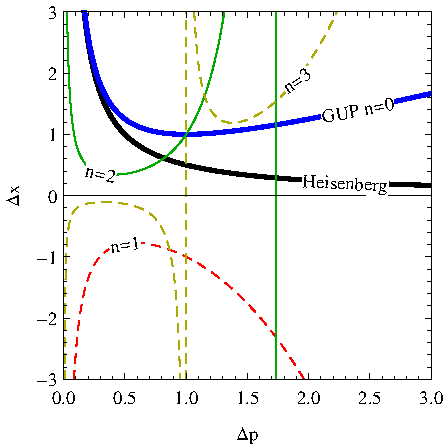
\includegraphics[scale=1]{figures/gup-mod-mod.pdf}
\end{subfigure}
\begin{subfigure}{0.5\textwidth}
\caption{Ordinary modified GUP (sec. \ref{sec:2})}\label{fig:gup2}
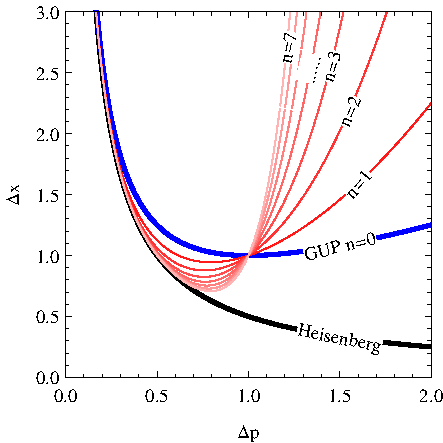
\includegraphics[scale=1]{figures/gup-mod.pdf}
\end{subfigure}
}% textbox
\caption{GUP modifications in comparison with ordinary uncertainity principle ($f(p)=0$), ordinary GUP in 4d ($f(p)=p^2$). Here, $\beta=L=1$. The pictures actually shows the function $x = \frac{1 + f(p)}{2 p}$.
}\label{fig:gup}
\end{figure}
%
\subsection{The modified GUP}
From $\C A^{-2}$ we get the modified GUP expression by backwards following Kempf's integral measure
\begin{equation}
\C A^{-2} \delta(x) = \int \frac{\d^N p}{1 + f(\bv p)}
\end{equation}
This function $f(p)$ is the one that enters the GUP as
\begin{equation}
\Delta x \Delta p \geq \frac \hbar2 (1 + f(p))
\end{equation}
So we just insert
\begin{equation}
\highlight{
f(p) = \frac 1{\C A^{-2}(p)} - 1
=
\frac{(-1)^N}{(N-3)!}
\frac{2 i p \beta}{\left(1+i\sqrt{\beta} p\right)^{-(N-2)} - \left(1-i\sqrt{\beta} p\right)^{-(N-2)} }.
}%eoh
\end{equation}
For $N=3$, this gives the well-known $f(p)=\beta p^2$, while for example for $N=4$, the GUP is given by
\begin{equation}
\Delta x \Delta p \geq \frac{\hbar}2 \left(
p^2 \beta^2 - \frac{1}{2}
\right),
\end{equation}
while for $N=5$, things get even worse
\begin{equation}
\Delta x \Delta p \geq \frac \hbar2 \left(
\frac{(1 + p^2 \beta)^3}{6 - 2 p^2 \beta}
\right).
\end{equation}
It seems that those expressions does not reduce to the ordinary Heisenberg principle for small $p$ (or rather $\beta$). The minimal length picture is also lost, as the relationship is for non-even $n$ negative and thus physically meaningless. See  figure \ref{fig:gup1} for a plot for the first extra dimensions $n=N-3$ in the $\Delta x \Delta p$ plane.

\newpage
\section{Weak-field approximation of the ordinary modified GUP}\label{sec:2}
\begin{figure}
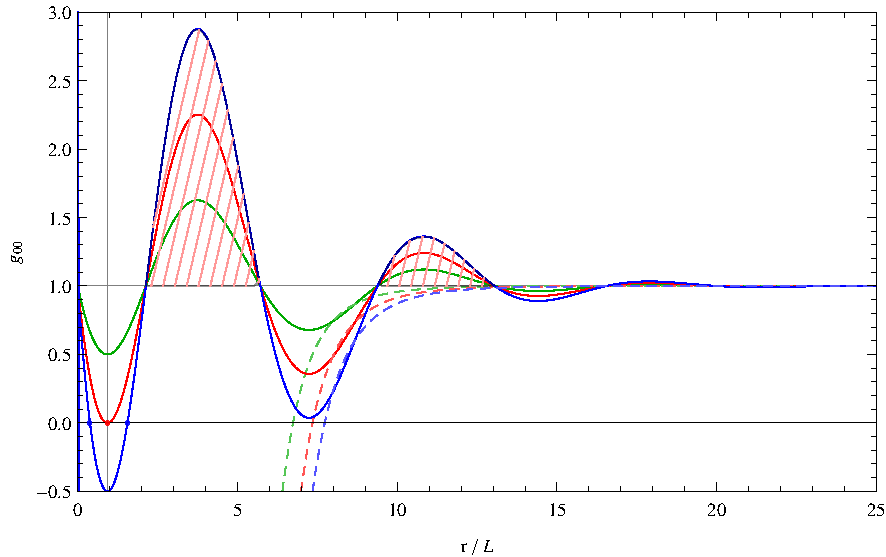
\includegraphics[scale=1]{figures/g00-GUP-n5.pdf}
\caption{The modified GUP metric in $n=5$ large extra dimensions exhibits three notable repulsive spheres, defined by $g_{00}>1$ and shaded red in this plot. Since the wiggling is exponentially surpressed with increasing radius, c.f. \eqref{eq:res}, repulsive regions do not appear at bigger distances, that is, the Schwarzschild limit holds. Anyway, the shown metric differs heavily from the Schwarzschild limit already $r=17L$.}\label{fig:mod-GUP}
\end{figure}
In this section, we again consider the \emph{original} modified GUP proposed by Sven in April 2014. It reads  in $n=N-3$ large extra dimensions ($p=|\bv p|$):
%
\begin{equation}
[x^i, p_j] = i \delta^i_j (1 + L^{2+n} p^{2+n}),
\end{equation}
%
see figure \ref{fig:gup2} for a plot of the corresponding GUP $\Delta x \Delta p \geq \frac{\hbar}{2}(1+f(p))$. Sven found that this approach produces smeared matter densities that induce metrics exposing repulsive zones (thick spheres around the Black Hole, see figure \ref{fig:mod-GUP}) at short scales. This is based on the fluctuating matter density that predicts ranges of negative matter density due to the cosine terms, as derived in \emph{Calc18} and approved by Maximiliano:
\begin{equation} \label{eq:res}
\C T^0_0 \approx 
\sum_{\varphi \in \Phi_n} e^{-\nicefrac rL \sin(\varphi)} \cos\left( \nicefrac rL \cos(\varphi) \right).
\end{equation}
It is worth investigating the limits of the theories. This is done by taylor expansions. We could for example investigate the long-distance behaviour of the lower Gamma function that appears in the gravitational potential $V(r) = 1-g_{00}$,
\begin{equation}\label{eq:gamma-approx}
\lim_{z\to \infty} \gamma(n, z) = e^{-z} z^n \left(
\frac 1z + \frac n{z^2} + \C O\left( \frac 1{z^3} \right) \right).
\end{equation}
I didn't yet compute these limits because they were clearly visible at the figures in \emph{Calc18} (or e.g.\ figure \ref{fig:mod-GUP}), as the proposed Black Holes always have a clear Schwarzschild/flat space limit.

In September, P.N. proposed investigating the limits of the nonlocal operator $\C A$, which means in the derivation of the GUP metric \cite{work} at the \emph{start} of the calculation, not at the \emph{end}. In practical terms this means approximating the deformed matter density
\begin{equation}\label{eq:rho}
\C T^0_0 = \frac{M}{(2\pi)^N}
\int \frac{\d^N p}{1 + L^{2+n} p^{2+n}} e^{i \bv x \cdot \bv p},
\end{equation}
with a series expansion of the nonlocal action, using the well-known identities
\begin{align}\label{eq:series1}
\lim_{x\to 0} \frac{1}{1+x} &= 1 - x + x^2 + \C O(x^3)
\\
\text{and}\quad
\lim_{x\to \infty} \frac 1{1+x} &= \frac 1x - \frac 1{x^2} + \C O\left( \frac 1{x^3} \right).
\end{align}
With the rule of thumb ``\emph{big momenta correspond to small distances}'' in mind, we investigate the limit
\begin{equation}\label{eq:PN-limit}
\highlight{
\lim_{p\to 0} \frac{1}{1+L^{N-1}p^{N-1}} = 1 - L^{N-1} p^{N-1} + \C O(p^2)
}% eoh
\end{equation}
which corresponds to far distances from the black hole, i.e. the Schwarzschild limit, with a first order correction term. We could also interpret this limit in terms of $L\to 0$, that is, $\beta \to 0$, or say that we expand the GUP effects \emph{around} the Schwarzschild solution.

\begin{figure}
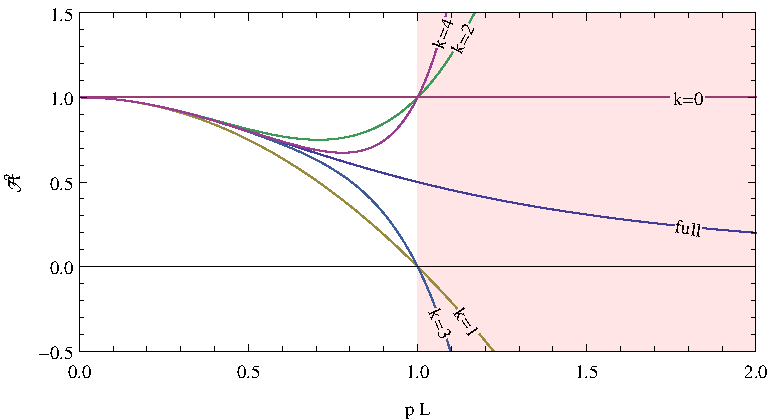
\includegraphics[scale=1]{figures/conv-radius.pdf}
\caption{Plot of the $k$. series approximation of $\C A^{-2}=1/(1+(Lp)^{2+n})$ for an arbitrary extra dimension $n$ (here $n=0$), as given in equation \eqref{eq:PN-limit}. The convergence radius for the series is always $L$, that is, the approximation breaks down for $r>L$ (red area). As these functions are the amplitude for the fourier coefficients, this motivates truncating the fourier transformation \eqref{eq:Twannabe} to the interval $p \in [-L,L]$.}\label{fig:conv}
\end{figure}

It turns out that this expansion is not only an exercise like tayloring the gamma \eqref{eq:gamma-approx} in $V(r)$, but requires a special treatment of the divergences. Consider the approach just inserting the first two orders of the approximation \eqref{eq:PN-limit} into the matter density \eqref{eq:rho}:
\begin{align}\label{eq:Twannabe}
\C T^0_0 &\approx
 \frac{M}{(2\pi)^N}
\int \d^N p~ e^{i \bv x \cdot \bv p}
+ 
\frac{M L^{N-1}}{(2\pi)^N}
\int \d^N p~p^{N-1} e^{i \bv x \cdot \bv p}
\\
&= M \delta(x)
+ 
\frac{M L^{N-1}}{(2\pi)^N}
\int \d^N p~p^{N-1} e^{i \bv x \cdot \bv p}.
\end{align}
We see that this integral diverges for $N>1$. This is not surprising as integrating a truncated taylor series with finite convergence radius $p_c$ over the full space is always diverging. Defining the series as (with $m=N-1$)
\begin{equation}\label{eq:def-series}
\C A^{-2}(p) := \frac{1}{1 + (L p)^m}
= \lim_{k\to\infty} \sum_{n=0}^k (-1)^n (Lp)^{n m}
\end{equation} 
allows directly reading the series coefficients $c_n=(-1)^n L^{nm}$ and determining the convergence radius, as shown in figure \ref{fig:conv} as the red shaded region:
\begin{equation}
p_c=\lim \left| \frac{c_{n+1}}{c_n}\right| = \lim \left| \frac{\pm L^{m(n+1)}}{\mp L^{mn}} \right| = L^m.
\end{equation}

We present here two methods how to deal with the divergence: Regularisation (section \ref{sec:reg}) and another approach of deriving the matter density, inspired by Kempfs Delta representations (section \ref{sec:kempf}). In both approaches, we work with the effective one dimensional integral, which is basically the same formalism as in section \ref{sec:nonlocal-backward}. Since the following section, the fourier transformation direction reversed in respect to section \ref{sec:nonlocal-backward}, the effective kernel for an approximation of order $k$ is given by
%
\begin{equation}\label{eq:veff2}
v(p) = - \frac{\Omega_N}{2 L^N} \frac{i}{z} q^{N-2} \left[
\sum^k_{n=0} (-1)^n q^{n m} \Theta(p) +
(-1)^{N+1}\sum^k_{n=0} (-1)^n (-q)^{n m} \Theta(-p) \right].
\end{equation}
with dimensionless units $q=LP$, $z=r/L$ and the shorthand $m=N-1$. $\Omega_N$ collects propertionality factors like $2\pi$ which will be neglected here.

\subsection{Regularized Fourier transformation}\label{sec:reg}
Accepting the fact of a finite convergence radius of the $\C A^{-2}$ series expansion motivates to handle the infinities by limiting the fourier transformation \eqref{eq:rho} in a way that, in 1 dimension, with \eqref{eq:veff2},
\begin{equation}\label{eq:finite1}
\int_{-\infty}^\infty 
\left(1 - q^m + q^{2m} + \C O(q^3)\right)
\d q~q^{m-1}~e^{i z q}
\to 
\int_{-a}^a
\left(1 - q^m + q^{2m} + \C O(q^3)\right)
\d q~q^{m-1}~e^{i z q}.
\end{equation}
%
Identifying $a=L$ would be appealing, but allows no more checking the effects of the truncation, because $a\to \infty$ would then also mean $L\to \infty$. In dimensionless coordinates, as used in eq \eqref{eq:finite1}, $a \leq 1$ is the meaningful domain where divergences due to the series truncation are suppressed.

The boxing causes serious difficulties in the interpretation of the results. Consider the most simple case $k=1$ and $N=3$, that is, the Dirac Delta
\begin{equation}
\int_{-\infty}^\infty e^{i \bv x \cdot \bv p} \d^3 p = \delta^3(\bv x)
\end{equation}
in the ``boxed volume $a$'', more precisely the $N$-sphere with radius $a$, called $\C B(a)$, gets
\begin{equation}\label{eq:delta-approx}
\int_{\C B(a)} e^{i \bv x \cdot \bv p} \d^3 p = 
\frac{\Omega_N}{2 L^3} \frac{i}{z} \int_{-a}^a
q~e^{ipz} \d q = 
\frac{\Omega_N}{2 L^3} \frac{i}{z^3}
\left( \Gamma(2, iaz) - \Gamma(2, -iaz) \right),
\end{equation}
with the upper gamma function $\Gamma(a,x) = \int_x^\infty t^{a-1} e^{-t} \d t$, which shall be treated in a box with (dimensionless) extend $a \leq 1$, c.f. figure \ref{fig:delta}. Evventually for $a\to\infty$, equation \eqref{eq:delta-approx} is a delta approximation.

\begin{figure}
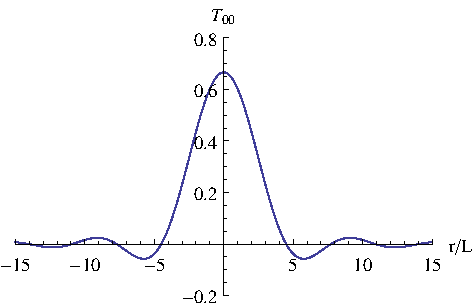
\includegraphics[scale=1]{figures/delta-box.pdf}
\caption{The ``sharpest object'' in an $a=L$ box: Plot of equation \eqref{eq:delta-approx}.}\label{fig:delta}
\end{figure}

\begin{figure}[h!]
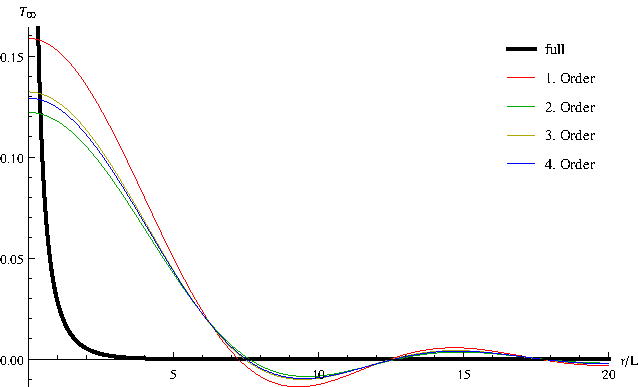
\includegraphics[scale=1]{figures/t00-regularized.pdf}
\caption{$\C T_{00}/(M/L^3)$ in approximations of $k$. order. The red line corresponds to the dirac delta (fig \ref{fig:delta}), while the next orders give nonlocal corrections. For $k\to \infty$, the full form as derived in \cite{isi2013} shall be arrived. Actually I didn't compute the full result in the limited volume $a<\infty$, so $k\to\infty$ will clearly be not be identical to the black curve.}\label{fig:T00-regularized}
\end{figure}
%
As we expect for more and more orders $k$ in the series \eqref{eq:def-series} the non-local effects to appear, we expect the first order ($k=0$) term, as shown in \eqref{eq:delta-approx}, to be the \emph{sharpest} and most-Dirac-like object. But regarding figure \ref{fig:delta}, the graph of this function already shows wiggling around $T_{00}=0$. The failure of this Ansatz is already encoded here.

It is easy to compute the $\C T_{00}$ terms for the $k$. order by partial integration. Figure \ref{fig:T00-regularized} shows some results. Qualitatively, the 2. to 4. order change really few (not to say nothing) on the Delta disaster. We cannot identify the source of nonlocal effects in this figure. This approach tells us \emph{nothing}.

\subsection{The Kempf representation}\label{sec:kempf}
In this final section we choose another approach to solve an integral like \eqref{eq:Twannabe}, which follows Kempfs Delta distribution representations~\cite{Kempf2014} from 2014. He proposes writing
\begin{equation}\label{eq:kempf1}
\delta(x) = \frac{1}{\sqrt{2\pi}} \frac{1}{g(-i\partial_x)} \tilde g(x),
\end{equation}
with a ``suitably well-behaved'' function $g(x)$ and it's fourier transformed $\tilde g(x)$. Note that in the Kempf paper, function arguments are taken literally as \emph{placeholders} (slots), so one must not be confused that $\tilde g(x)$ and $\tilde g(y)$ describe the same function with different arguments putted in.

The authors of \cite{Kempf2014} quickly extend their formalism on functionals. In this spirit, we extend it to extra dimensions, where the delta representation reads
\begin{equation}
\delta^N(\bv x) = \frac{1}{(2\pi)^{\nicefrac N2}}
\frac{1}{g(-i \nabla_{\bv x})} \tilde g(\bv x)
\end{equation}

By following Kempfs brave recasting of the dirac delta \eqref{eq:kempf1}, we get a ``new'' representation of the $N$-dimensional Fourier transformation
\begin{equation} \label{eq:gtilde}
\highlight{
\tilde g(\bv x) = (2\pi)^{\frac N2} g(-i\nabla_{\bv x}) \delta^N(\bv x).
}%eoh
\end{equation}
When choosing $g(|\bv p|)=\C A^{-2}(p)=1/(1+(pL)^{N-1})$, this looks very much as the well-known starting point for the nonlocal action on the Dirac delta,
\begin{equation} \label{eq:T00kempf}
\C T^0_0 = \frac{M}{A_{N-1} r^{N-1}} \C A^{-2}(\square) \delta(\bv x),
\end{equation}
where there is a mismatch with $\sqrt{\square_{\bv x}} \leftrightarrow -i \nabla_{\bv x}$. This shall be ignored at this point.

Basically, the authors of \cite{Kempf2014} propose new methods how to solve an equation like \eqref{eq:T00kempf}: Instead of going to momentum space to get the action of the operator, they propose to solve such equations in pure position space, by letting the differential operator act on a delta representation. This might be the gaussian approximation
\begin{equation}
\delta_\sigma(r) = \frac{1}{\sqrt{2\pi}\sigma} \exp \left( - \frac{r^2}{2\sigma^2} \right),
\quad \delta(r) = \lim_{\sigma\to 0} \delta_\sigma(r).
\end{equation}
Now we can compute the $k$. matter density approximation by derivation:
\begin{equation}
\C T^0_0 =
\frac{M}{A_{N-1} r^{N-1}}
\frac{1}{\sqrt{2\pi} \sigma}
\sum_{n=0}^k (-1)^n (-iL)^{mn} \nabla_{\bv x}^{mn}
\exp\left( -\frac{|\bv x|^2}{2 \sigma^2} \right)
\end{equation}
The $k=0$ and $k=1$ results are shown in figure \ref{fig:kempf1}. In contrast to the regularisation approach \ref{sec:reg}, this looks probabily more appealing.

Integrating up these results to a unit mass distribution $\C M=\int_0^r \C T^0_0(r') r'^{N-1} \d r$ and composing the Schwarzschild metric gives figure \ref{fig:kempf2}. This is our final result in this document.

\begin{figure}
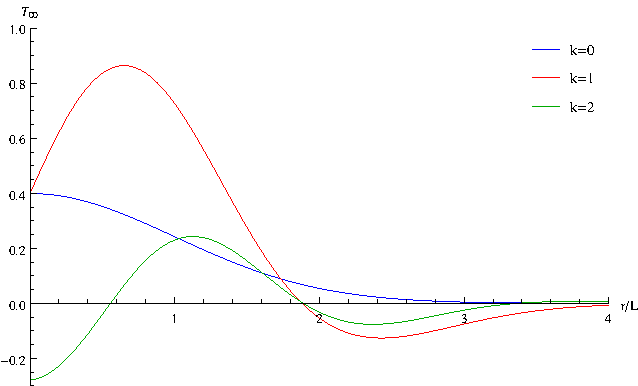
\includegraphics[scale=1]{figures/t00-kempf.pdf}
\caption{The lower order approximations of $\C T_{00}/(M/L^3)$ with the Kempf approach, for $N=3$, $\sigma=1$. Smaller $\sigma$ make a better Delta approximation.}\label{fig:kempf1}
\end{figure}

\begin{figure}
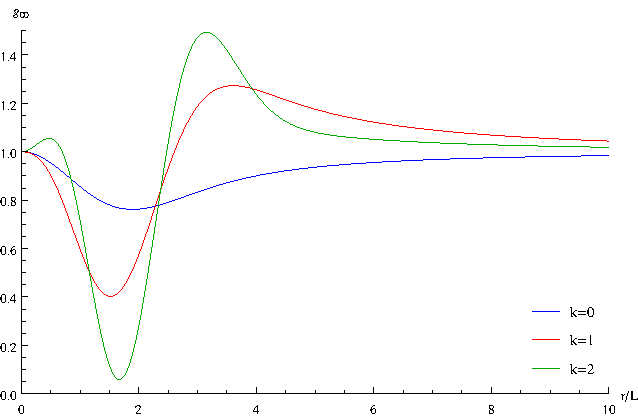
\includegraphics[scale=1]{figures/g00-kempf.pdf}
\caption{The metric in $k$. order approximation of the nonlocal operator, using the Kempf approach. This plot is in $N=4$ dimensions, with ``unit mass'' $M=1$ and $\sigma=1$.}\label{fig:kempf2}
\end{figure}

\newpage
\phantom{bla} % for making the Refs move to the bottom

\vfill
\begin{thebibliography}{}
\bibitem{work}
  M.~Isi, M.~Knipfer, J.~Mureika and P.~Nicolini,
  ``Self-Completeness and the Generalized Uncertainty Principle in Extra Dimensions,'' \textit{in progress} (my latest copy: April 26, 2014).
  
\bibitem{kempf1995}
  A.~Kempf, G.~Mangano and R.~B.~Mann,
  ``Hilbert space representation of the minimal length uncertainty relation,''
  Phys.\ Rev.\ D {\bf 52} (1995) 1108
  [\href{http://arxiv.org/abs/hep-th/9412167}{hep-th/9412167}].

\bibitem{isi2013}
  M.~Isi, J.~Mureika and P.~Nicolini,
  ``Self-Completeness and the Generalized Uncertainty Principle,''
  JHEP {\bf 1311} (2013) 139
  [\href{http://arxiv.org/abs/arXiv:1310.8153}{arXiv:1310.8153 [hep-th]}].
  
  
\bibitem{NS2012}
  P.~Nicolini and E.~Spallucci,
  ``Holographic screens in ultraviolet self-complete quantum gravity,''
  Adv.\ High Energy Phys.\  {\bf 2014} (2014) 805684
  [\href{http://arxiv.org/abs/arXiv:1210.0015}{arXiv:1210.0015 [hep-th]}].
  
\bibitem{Rizzo}
  T.~G.~Rizzo,
  ``Noncommutative Inspired Black Holes in Extra Dimensions,''
  JHEP {\bf 0609} (2006) 021
  [\href{http://arxiv.org/abs/hep-ph/0606051hep-ph/0606051}{arXiv:hep-ph/0606051}].
  %%CITATION = HEP-PH/0606051;%%
  %100 citations counted in INSPIRE as of 29 Aug 2014

\bibitem{Kempf2014}
  A.~Kempf, D.~M.~Jackson and A.~H.~Morales,
  ``New Dirac Delta function based methods with applications to perturbative expansions in quantum field theory,''
  [\href{http://inspirehep.net/record/1288521}{InSpire}] [\href{http://arxiv.org/abs/1404.0747}{arXiv:1404.0747 [math-ph]}].
  See also Marcos Talk \href{https://fias.uni-frankfurt.de/~koeppel/journalclub/ss2014/14-07-30/slides-dirac-delta.pdf}{New Dirac Delta representation} (30. July 2014)
  %%CITATION = ARXIV:1404.0747;%%


\end{thebibliography}

\end{document}
